\documentclass[10pt,aspectratio=1610]{beamer} % use option aspectratio=169 or 1610 for wide slides
% Note: For online presentations via Zoom use the ratio of the screen you want to share
\usetheme{Rochester}

% load Syscop style
\usepackage{style/syscop}
\usepackage{booktabs}
\usepackage{enumitem}
%--------------------------------------------------
% TITLE
%--------------------------------------------------

% NOTE: what's in [ ] goes to the footer for the fields title, author and date
% \begin{frame}{MPC for trajectory following AGVs}
\title[Model Predictive Control for trajectory following Automated Guided Vehicles]{\large Model Predictive Control for trajectory following Automated Guided Vehicles}
% \subtitle{\normalsize Master Thesis}
\author[\large Akash John Subash]{\large Akash John Subash}
\institute{\large Systems Control and Optimization \& ek robotics}
\date[\today]{\\ \today }
% \end{frame}


%--------------------------------------------------
% Useful packages
%--------------------------------------------------
\usepackage{amsmath}
\usepackage{mathtools}
\usepackage{graphicx}
\usepackage{hyperref}
\usepackage{optidef}
\usepackage{xcolor}
\usepackage{upgreek}
\usepackage[euler]{textgreek}
\usepackage{appendixnumberbeamer}
% \hypersetup{
%     colorlinks=true,
%     linkcolor=blue,
%     filecolor=blue,      
%     urlcolor=blue,
%     pdftitle={Overleaf Example},
%     pdfpagemode=FullScreen,
%     }
\setbeamertemplate{footline}[frame number]
% TODO make title page same aspect ratio as others?
% TODO place EK and ufr logos beside each other (coloumns)
\begin{document}
\InsertTitle
% \titlepage


\begin{frame}{Overview}
	\large{Objective : Trajectory tracking MPC with obstacle avoidance on a real AGV.}
	\hfill \break
	\begin{itemize}[label=\textbullet]\large
		\item Tricycle kinematics
		\item Obstacle modelling
		\item OCP formulations
		\item Gazebo tests
		\item Warehouse tests
	\end{itemize}
\end{frame}

% \begin{frame}{Objective}
% 	Objective : Trajectory tracking MPC deployment with obstacle avoidance on a real \ac{AGV}
% \end{frame}

\begin{frame}{AGV description}
\begin{columns}[onlytextwidth]
	\begin{column}{0.5\textwidth}
			\begin{center}
			\def\svgwidth{1\textwidth}
			\input{figures/agv_dim.pdf_tex}
			\end{center}
	\end{column}
	\begin{column}{0.5\textwidth}
		\begin{table}[h!tbp]
			\small
			\begin{center}
				\begin{tabular}{lccccl}\toprule
					\textbf{Quantity} & \textbf{Value}\\
					\midrule
					length $l_{\mathrm{agv}}$ & $\mathrm{2.914\,m}$\\
					breadth $b_{\mathrm{agv}}$ & $\mathrm{1.115\,m}$\\
					height $h_{\mathrm{agv}}$ & $\mathrm{2.238\,m}$\\
					weight $w_{\mathrm{agv}}$ & $\mathrm{3.7\cdot10^{3}\,kg}$\\
					\bottomrule
				\end{tabular}
			\end{center}
		\end{table}
	\end{column}
\end{columns}
\end{frame}

\begin{frame}{Position tracking Cartesian model}
	\begin{columns}[onlytextwidth]
		\begin{column}{0.5\textwidth}
			\begin{center}
			\def\svgwidth{1.0\textwidth}
			\input{figures/kin_cart2.pdf_tex}
			\end{center}
		\end{column}
		\begin{column}{0.5\textwidth}
			\begin{align*}
				\dot{\zeta^{p}}(t) = \begin{bmatrix}
					\dot{x}\\
					\dot{y}\\
					\dot{\varphi}\\
					\dot{v}\\
					\dot{\alpha}\\
				\end{bmatrix} & = 
				\begin{bmatrix}
					v\, \cos(\alpha)\, \cos(\varphi)\\
					v\, \cos(\alpha)\, \sin(\varphi)\\
					\dfrac{v}{d}\, \sin(\alpha)\\
					a\\
					\omega 
				\end{bmatrix}
			\end{align*}
		
		\begin{itemize}[label=\textbullet]
			\item State ${\zeta^{p}}^T$:= $[{\zeta^{c}}^T,\,{\zeta^{u}}^T]$
			\item Vector $\zeta^{c}$: Cartesian position $(x,\, y)$,\\
			\hspace{0.62in} heading $\varphi$
			\item Vector $\zeta^{u}$: wheel speed $v$,\\ 
			\hspace{0.62in} wheel orientation $\alpha$
		\end{itemize}
		\end{column}
	\end{columns}
\end{frame}

\begin{frame}{Trajectory tracking Frenet model}
	\begin{columns}[onlytextwidth]
		\begin{column}{0.5\textwidth}
			\begin{center}
			\def\svgwidth{1.0\textwidth}
			\input{figures/kin_fren2.pdf_tex}
			\end{center}
		\end{column}
		\begin{column}{0.5\textwidth}
		\begin{align*}
			\dot{\zeta^{d}}(t) = \begin{bmatrix}
			\dot{s}\\
			\dot{n}\\
			\dot{\beta}\\
			\dot{v}\\
			\dot{\alpha}\\
		\end{bmatrix} &= 
		\begin{bmatrix}
			\dfrac{v\, \cos(\alpha)\, \cos(\beta)}{1 - n\, \kappa(s)}\\
			v\, \cos(\alpha)\, \sin(\beta)\\
			\dfrac{v}{d}\, \sin(\alpha) - \dfrac{\kappa(s)\, v\, \cos(\alpha)\, \cos(\beta)}{1 - n\, \kappa(s)}\\
			a\\
			\omega 
		\end{bmatrix}
		\end{align*}
		\begin{itemize}[label=\textbullet]
			\item State ${\zeta^{d}}^T$:= $[{\zeta^{f}}^T,\,{\zeta^{u}}^T]$
			\item Vector $\zeta^{f}$: track progress $s$,\\ 
			\hspace{0.62in} lateral displacement $n$,\\ 
			\hspace{0.62in} track orientation $\beta$
		\end{itemize}
		\end{column}
	\end{columns}
\end{frame}

\begin{frame}{Comparison of Cartesian, Frenet frames}
	\begin{columns}[onlytextwidth]
		\begin{column}{0.5\textwidth}
				Cartesian
				\begin{itemize}[label=\textbullet]
					\item Intuitive geometric constraint representation
					\item No observer needed in the feedback path
					\item Jumps in cost during set point tracking. 
				\end{itemize}
		\end{column}
		\begin{column}{0.5\textwidth}
				Frenet
				\begin{itemize}[label=\textbullet]
					\item Smooth trajectory tracking cost
					\item Intuitive curve representation
					\item No convexity guarantees for transformed convex Cartesian obstacle shape
				\end{itemize}
		\end{column}
	\end{columns}
\end{frame}

\begin{frame}{Trajectory tracking lifted Frenet model}
	\begin{columns}[onlytextwidth]

		\begin{column}{0.5\textwidth}
		\begin{align*}
			\dot{\zeta^{l}}(t) = 
			\begin{bmatrix}
				\dot{x}\\
				\dot{y}\\
				\dot{\varphi}\\
				\dot{s}\\
				\dot{n}\\
				\dot{\beta}\\
				\dot{v}\\
				\dot{\alpha}\\
			\end{bmatrix} &= 
			\begin{bmatrix}
				v\, \cos(\alpha)\, \cos(\varphi)\\
				v\, \cos(\alpha)\, \sin(\varphi)\\
				\dfrac{v}{d}\, \sin(\alpha)\\
				\dfrac{v\, \cos(\alpha)\, \cos(\beta)}{1 - n\, \kappa(s)}\\
				v\, \cos(\alpha)\, \sin(\beta)\\
				\dfrac{v}{d}\, \sin(\alpha) - \dfrac{\kappa(s)\, v\, \cos(\alpha)\, \cos(\beta)}{1 - n\, \kappa(s)}\\
				a\\
				\omega
			\end{bmatrix}
		\end{align*}
		\end{column}
		\begin{column}{0.5\textwidth}
		\begin{align*}
			u(t) &= 
			\begin{bmatrix}
				a \\
				\omega
			\end{bmatrix}\\
		\end{align*}
		\begin{itemize}[label=\textbullet]
			\item State ${\zeta^{l}}^T$:= $[{\zeta^{c}}^T,\,{\zeta^{f}}^T,\,{\zeta^{u}}^T]$
			\item Control $u$: wheel acceleration $a$,\\
			\hspace{0.62in} wheel turning rate $\omega$
		\end{itemize}
		\end{column}
	\end{columns}
\end{frame}

\begin{frame}{Trajectory tracking lifted Frenet model}
	\begin{columns}[onlytextwidth]
		\begin{column}{0.5\textwidth}
			\begin{itemize}[label=\textbullet]
				\item Frenet differential state ${\zeta}^{f}$
				\item Cartesian algebraic state $\tilde{\zeta}^{c}$
				\item DAE Index-1 reduction: 
			\end{itemize}
		\begin{align*}
					\begin{split}
					\dot{\zeta}^{c} &= \dfrac{d{\mathcal{F}^{-1}_{\upgamma}(\zeta^{f})}}{dt}\\
					&= \dfrac{\partial{\mathcal{F}^{-1}_{\upgamma}(\zeta^{f})}}{\partial{\zeta}^{f}}\,f(\zeta^{f}, u)\\
					&= \begin{bmatrix}
						v\, \cos(\alpha)\, \cos(\varphi)\\
						v\, \cos(\alpha)\, \sin(\varphi)\\
						\dfrac{v}{d}\, \sin(\alpha)
					   \end{bmatrix}
					\end{split}
				\end{align*}
		\end{column}

		\begin{column}{0.5\textwidth}
			Cartesian-Frenet transforms:
			\begin{mini}|l|
				{s}{ \lVert p_{\mathrm{agv}} - \upgamma^{p}(s) \rVert^{2}_{2}}{s^{*} = }{}{{\label{Sopt}}}{}\nonumber
			\end{mini}

			\begin{align*}
				\zeta^{f} = \mathcal{F}_{\upgamma}(\zeta^{c}) &=\begin{bmatrix}
					s^{*}\\
					(p_{\mathrm{agv}} - \upgamma^{p}(s^{*}))\, e_{n}\\
					\varphi - \upgamma^{\varphi}(s^{*})
				\end{bmatrix} 
			\end{align*}
			
			\begin{align*}
				\zeta^{c} = \mathcal{F}^{-1}_{\upgamma}(\zeta^{f}) &=\begin{bmatrix}
					\upgamma^{x}(s) - n\, \sin( \upgamma^{\varphi}(s))\\
					\upgamma^{y}(s) + n\, \cos( \upgamma^{\varphi}(s))\\
					\upgamma^{\varphi}(s) + \beta
				\end{bmatrix} 
			\end{align*}
		\end{column}
	\end{columns}
\end{frame}

\begin{frame}{Operational Safety}
	\begin{columns}[onlytextwidth]
		\begin{column}{0.7\textwidth}
			\begin{center}
			\def\svgwidth{1.2\textwidth}
			\input{figures/breaking_distance.pdf_tex}
			\end{center}
		\end{column}

		\begin{column}{0.3\textwidth}
			\begin{itemize}[label=\textbullet]
				\item braking distance ${\delta}_{b}$
				\item AGV velocity $v_{agv}$
				\item AGV decelerration $a_{agv}$
			\end{itemize}
		\begin{align*}
			\delta_{b} = \dfrac{-v^{2}_{\mathrm{agv}}}{2\,a_{\mathrm{agv}}}
		\end{align*}
		\end{column}
	\end{columns}
\end{frame}

\begin{frame}{Covering circles}
	\begin{columns}[onlytextwidth]
		\begin{column}{0.45\textwidth}
			\begin{center}
			\def\svgwidth{1.1\textwidth}
			\input{figures/agv_3c2.pdf_tex}
			\end{center}
		\end{column}

		\begin{column}{0.45\textwidth}
		\begin{itemize}[label=\textbullet]
			\item 2D rotation matrix $M(\theta)$
			\item ${i} \in [1, .., n_{ob}]$ elliptical obstacles
			\item ${j} \in [1, .., n_{c}]$ covering circles
			\item ${k} \in [1, .., N]$ shooting nodes
		\end{itemize}
		\begin{align*}
			\begin{bmatrix}
				\Delta x_{i, j, k}\\
				\Delta y_{i, j, k}
			\end{bmatrix}^T
			\Sigma_{i}
			\begin{bmatrix}
				\Delta x_{i, j, k}\\
				\Delta y_{i, j, k}
			\end{bmatrix} - 1 = 0
		\end{align*}
	
		\begin{align*}\Sigma_{i} =
			\mathrm{M}(\theta_{i})^T
				\begin{bmatrix}
					1/\lambda^{2}_{i} & 0\\
					0 & 1/\rho^{2}_{i}
				\end{bmatrix}
				\mathrm{M}(\theta_{i})
		\end{align*}
		\end{column}
	\end{columns}
\end{frame}

\begin{frame}{Direct Elimination Frenet OCP}
	\begin{mini!}|l|
		{u_0,\zeta^{d}_0,..,u_{N-1},\zeta^{d}_N}{ \lVert \zeta^{d}_{N} - \zeta^{d}_{N, \mathrm{ref}} \rVert^{2}_{Q_{N}}+ \sum_{k = 0}^{N-1} \lVert \zeta^{d}_{k}- \zeta^{d}_{k, \mathrm{ref}} \rVert^2_Q + \lVert u_k \rVert^2_R}{}{}
		\addConstraint{}{\quad \quad\zeta^{d}_0 - \bar{\zeta^{d}_0}}{=0}
		\addConstraint{}{\quad \quad\zeta^{d}_{k+1} - \phi(\zeta^{d}_k, u_k)}{=0,}{\quad k=0,\ldots,N-1}
		\addConstraint{\underline{u} }{\le \quad u_k}{\le \overline{u},}{\quad k=0,\ldots,N-1}
		\addConstraint{\underline{w} }{\le \quad v_{k}\, \cos(\alpha_k)}{\le \overline{w},}{\hspace{0.12in} k=0,\ldots,N-1} \label{constr_veh_vel}
		\addConstraint{\underline{\dot{\varphi}} }{\le \quad \frac{v_k}{d}\, \sin(\alpha_k)}{\le \overline{\dot{\varphi}},}{\quad k=0,\ldots,N-1} \label{constr_veh_omg}
		\addConstraint{- \infty }{\le \quad n_{k}\, \kappa(s_{k})}{\le 1,}{\hspace{0.15in} k=0,\ldots,N-1}\label{constr_proj_uniq}
		\addConstraint{1 }{\le \quad \lVert \textGamma_{\mathrm{def}}(\zeta^{d}_{k}) - p_{i,\,\mathrm{ob}} \rVert^{2}_{\Sigma_{i}(\cdot)}}{\le \infty,}{\hspace{0.1in} k=0,\ldots,N-1}\label{constr_obst_def}
		\addConstraint{}{}{\qquad\hspace{0.23in} i=0,\ldots,n_{\mathrm{ob}}-1}\nonumber
	\end{mini!}
\end{frame}

\begin{frame}{Lifted Frenet OCP}
	\begin{mini!}|l|
		{u_0,\zeta^{d}_0,..,u_{N-1},\zeta^{d}_N}{ \lVert \zeta^{d}_{N} - \zeta^{d}_{N, \mathrm{ref}} \rVert^{2}_{Q_{N}}+ \sum_{k = 0}^{N-1} \lVert \zeta^{d}_{k}- \zeta^{d}_{k, \mathrm{ref}} \rVert^2_Q + \lVert u_k \rVert^2_R}{}{}
		\addConstraint{}{\quad \quad\zeta^{f}_0 - \mathcal{F}_{\upgamma}(\zeta^{c}_0)}{=0}
		\addConstraint{}{\quad \quad\zeta^{d}_0 - \bar{\zeta^{d}_0}}{=0}
		\addConstraint{}{\quad \quad\zeta^{l}_{k+1} - \phi(\zeta^{l}_k, u_k)}{=0,}{\quad k=0,\ldots,N-1}
		\addConstraint{\underline{u}}{\le \quad u_k}{\le \overline{u},}{\quad k=0,\ldots,N-1}
		\addConstraint{\underline{w}}{\le \quad v_{k}\, \cos(\alpha_k)}{\le \overline{w},}{\hspace{0.12in} k=0,\ldots,N-1}\label{constr_vel_agv}	
		\addConstraint{\underline{\dot{\varphi}} }{\le \quad \frac{v_k}{d}\, \sin(\alpha_k)}{\le \overline{\dot{\varphi}},}{\quad k=0,\ldots,N-1}\label{constr_omega_agv}
		\addConstraint{- \infty}{\le \quad n_{k}\, \kappa(s_{k})}{\le 1,}{\hspace{0.15in} k=0,\ldots,N-1}
		\addConstraint{1}{\le \quad \lVert \textGamma_{\mathrm{lf}}(\zeta^{l}_{k}) - p_{i,\,\mathrm{ob}} \rVert^{2}_{\Sigma_{i}(\cdot)}}{\le \infty,}{\hspace{0.1in} k=0,\ldots,N-1}\label{constr_obst_lf}
		\addConstraint{}{}{\qquad\hspace{0.23in} i=0,\ldots,n_{\mathrm{ob}}-1}\nonumber
	\end{mini!}
\end{frame}

\begin{frame}{Evaluation}
	\begin{columns}[onlytextwidth]
		\begin{column}{0.6\textwidth}
			\begin{itemize}[label=\textbullet]
				\item centreline deviation:
			\end{itemize}
			\begin{align*}
				\varepsilon_{n,  \mathrm{avg}} = \dfrac{1}{M}\sum_{l=0}^{M} |n_{l}|
			\end{align*}
			\begin{itemize}[label=\textbullet]
				\item oscillation metric:
			\end{itemize}
			\begin{align*}
				\varepsilon_{z, \mathrm{osc}} = \sqrt{\dfrac{1}{M-2}\sum_{l=0}^{M-2} (z_{l+1} - 2z_{l} + z_{l-1})^2}
			\end{align*}
		\end{column}

		\begin{column}{0.4\textwidth}
			Gazebo validation:
			\begin{itemize}[label=\textbullet]
			\item[\textcolor{blue}{\textbullet}] Reference trajectories in Gazebo
			\item Delay compensation schemes
			\item OCPs for elliptical footprint
			\item[\textcolor{blue}{\textbullet}] OCPs for AGV covering circles
			\end{itemize}
			\hfill \break
			Warehouse validation:
			\begin{itemize}[label=\textbullet]
			\item[\textcolor{blue}{\textbullet}] OCPs for AGV covering circles
			\end{itemize}
		\end{column}
	\end{columns}
\end{frame}

\begin{frame}{Test track}
		\begin{center}
			\def\svgwidth{1\textwidth}
			\input{figures/agv_on_track.pdf_tex}
		\end{center}
\end{frame}

\begin{frame}{Trajectory reference comparison in Gazebo}
	\begin{table}[h!tbp]
		\small
		\begin{center}
			\begin{tabular}{lccccl}\toprule
				\textbf{Quantity} & \textbf{Value}\\
				\midrule
	
				Control weight $R$ & $[5$, $2.5\cdot10^{1}]$\\
				Terminal state weight $Q_{N}$ & $[10^{-1}$, $2.5\cdot10^{1}$, $10^{-8}$, $10^{-8}$, $5]$\\
				Ref1 state weight $Q$ & $[10^{-8}$, $2.5\cdot10^1$, $10^{-8}$, $10^{2}$, $10]$\\
				Ref2 state weight $Q$ & $[10^{2}$, $2.5\cdot10^1$, $10^{-8}$, $10^{-8}$, $10]$\\
				\bottomrule
			\end{tabular}
		\end{center}
		\caption{Weighting matrices in SI units}
	\end{table}
	
	\begin{align*}
		s_{k, \mathrm{ref}} &= s_{0} + \dfrac{s_{\mathrm{ref}}}{N}\,k \\
		v_{k, \mathrm{ref}} &= v_{\mathrm{ref}}
	\end{align*}
\end{frame}

\begin{frame}{Trajectory reference comparison in Gazebo}
	\begin{columns}[onlytextwidth]
		\begin{column}{0.75\textwidth}
		\begin{figure}[h!tbp]
			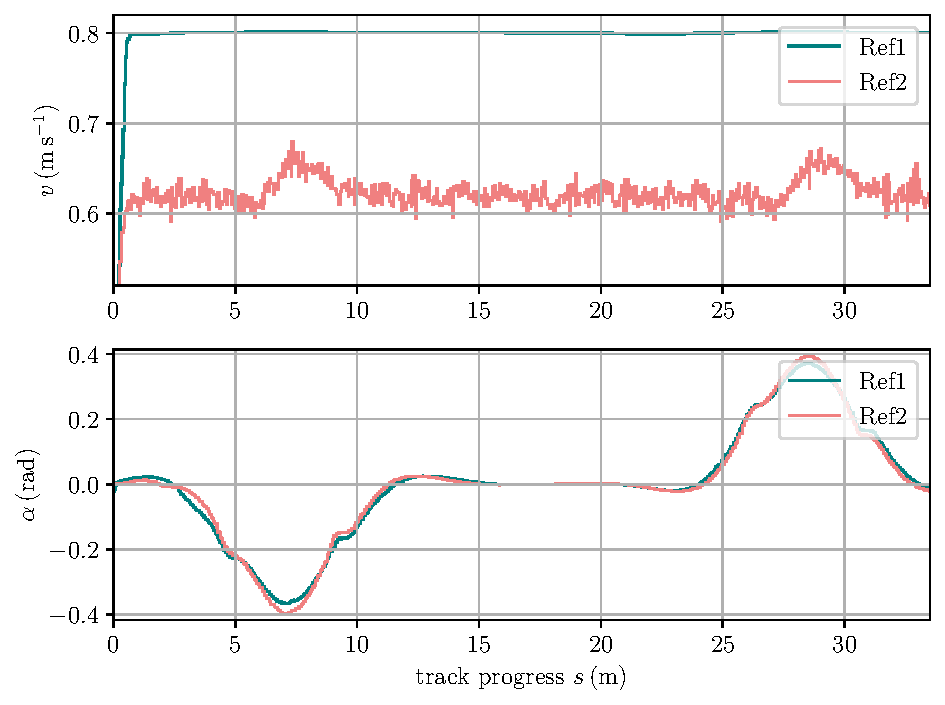
\includegraphics[scale=0.6]{figures/ucomp_ref.pdf}
		\end{figure}
		\end{column}

		\begin{column}{0.3\textwidth}
			\begin{table}[h!tbp]
				\small
				\begin{center}
					\begin{tabular}{lccccl}\toprule
						& $\varepsilon_{v, \mathrm{osc}}\,(\mathrm{m\,s^{-1}})$\\
						\midrule
						$\mathrm{Ref1}$& $4.26\cdot10^{-3}$\\
						$\mathrm{Ref2}$& $2.59\cdot10^{-2}$\\
						\bottomrule
					\end{tabular}
				\end{center}
			\end{table}
		\end{column}
	\end{columns}
\end{frame}

\begin{frame}{State $x,\,y$ comparison for AGV covering circles in Gazebo}
		\begin{figure}[h!tbp]
			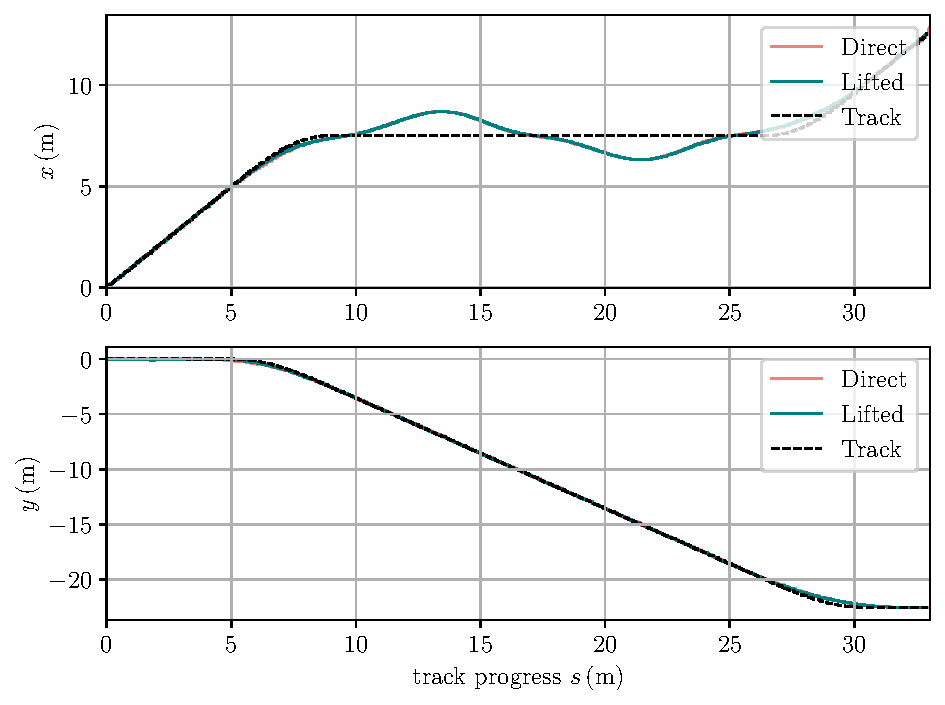
\includegraphics[scale=0.65]{figures/zeta_c10}
		\end{figure}

		% \begin{column}{0.3\textwidth}
		% 	\begin{table}[h!tbp]
		% 		\small
		% 		\begin{center}
		% 			\begin{tabular}{lccccl}\toprule
		% 				& $\varepsilon_{\n,\,\mathrm{avg}}\,(\mathrm{m})$\\
		% 				\midrule
		% 				$\mathrm{Direct}$& $5.1\cdot10^{-2}$\\
		% 				$\mathrm{Lifted}$& $5.0\cdot10^{-2}$\\
		% 				\bottomrule
		% 			\end{tabular}
		% 		\end{center}
		% 	\end{table}
		% \end{column}
\end{frame}

\begin{frame}{States $\varphi,\,n$ comparison for AGV covering circles in Gazebo}
	\begin{columns}[onlytextwidth]
	
	\begin{column}{0.75\textwidth}
			\begin{figure}[h!tbp]
			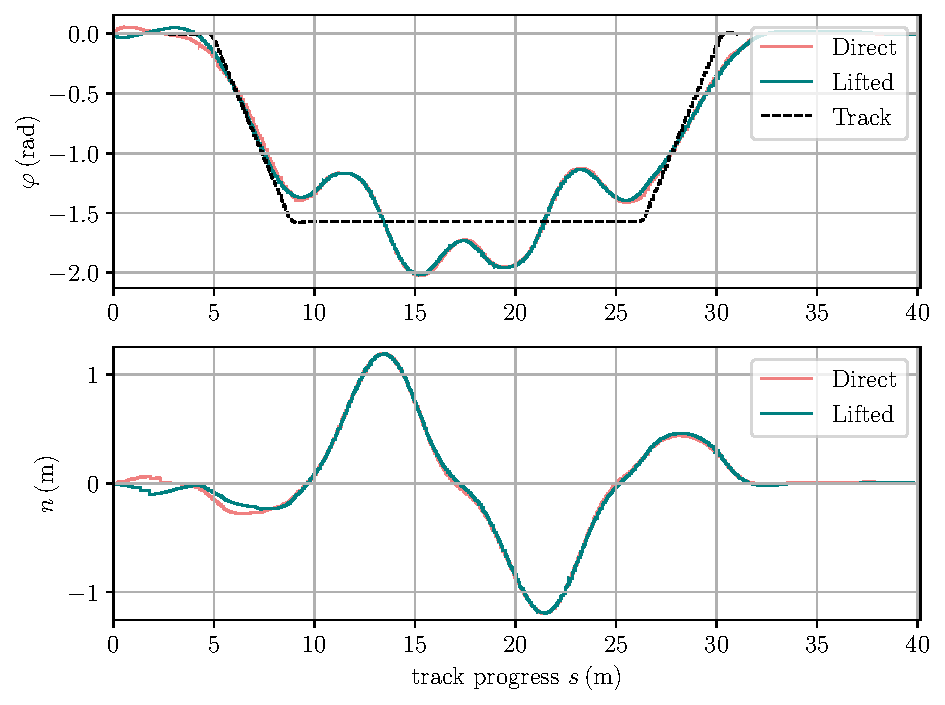
\includegraphics[scale=0.65]{figures/zeta_phi_n}
		\end{figure}
	\end{column}
	
	\begin{column}{0.3\textwidth}
		\begin{table}[h!tbp]
			\small
			\begin{center}
				\begin{tabular}{lccccl}\toprule
					& $\varepsilon_{n,\,\mathrm{avg}}\,(\mathrm{m})$\\
					\midrule
					$\mathrm{Direct}$& $5.10\cdot10^{-1}$\\
					$\mathrm{Lifted}$& $5.0\cdot10^{-1}$\\
					\bottomrule
				\end{tabular}
			\end{center}
			% \caption{Control oscillation metrics}
		\end{table}
	\end{column}
\end{columns}
\end{frame}

\begin{frame}{Control $u$ comparison for AGV covering circles in Gazebo}
\begin{columns}[onlytextwidth]
	\begin{column}{0.75\textwidth}
	\begin{figure}[h!tbp]
		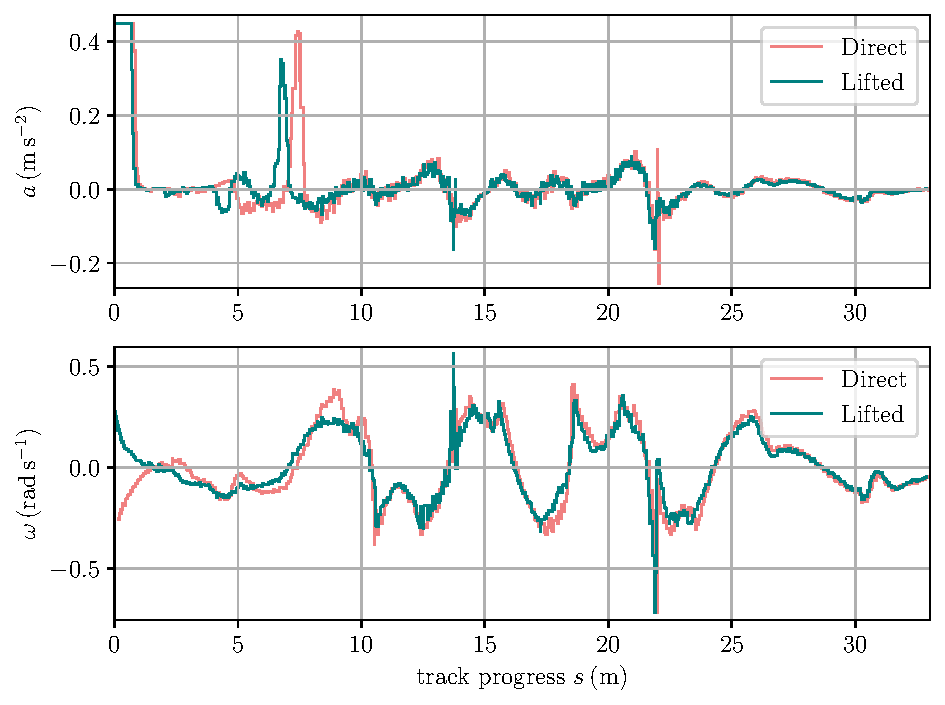
\includegraphics[scale=0.65]{figures/u}
		\end{figure}
	\end{column}
	\begin{column}{0.3\textwidth}
		\begin{table}[h!tbp]
			\small
			\begin{center}
				\begin{tabular}{lccccl}\toprule
					& $\varepsilon_{a,\,\mathrm{osc}}\,(\mathrm{m\,s^{-2}})$\\
					\midrule
					$\mathrm{Direct}$& $1.58\cdot10^{-2}$\\
					$\mathrm{Lifted}$& $1.56\cdot10^{-2}$\\
					\bottomrule
				\end{tabular}
			\end{center}
			% \caption{Control oscillation metrics}
		\end{table}

		\begin{table}[h!tbp]
			\small
			\begin{center}
				\begin{tabular}{lccccl}\toprule
					& $\varepsilon_{\omega,\,\mathrm{osc}}\,(\mathrm{rad\,s^{-1}})$\\
					\midrule
					$\mathrm{Direct}$& $1.57\cdot10^{-2}$\\
					$\mathrm{Lifted}$& $2.25\cdot10^{-2}$\\
					\bottomrule
				\end{tabular}
			\end{center}
			% \caption{Control oscillation metrics}
		\end{table}
	\end{column}
\end{columns}
\end{frame}

\begin{frame}{OCP comparison for AGV covering circles in Gazebo}
	\begin{columns}[onlytextwidth]
	\begin{column}{0.75\textwidth}
	\begin{figure}[h!tbp]
		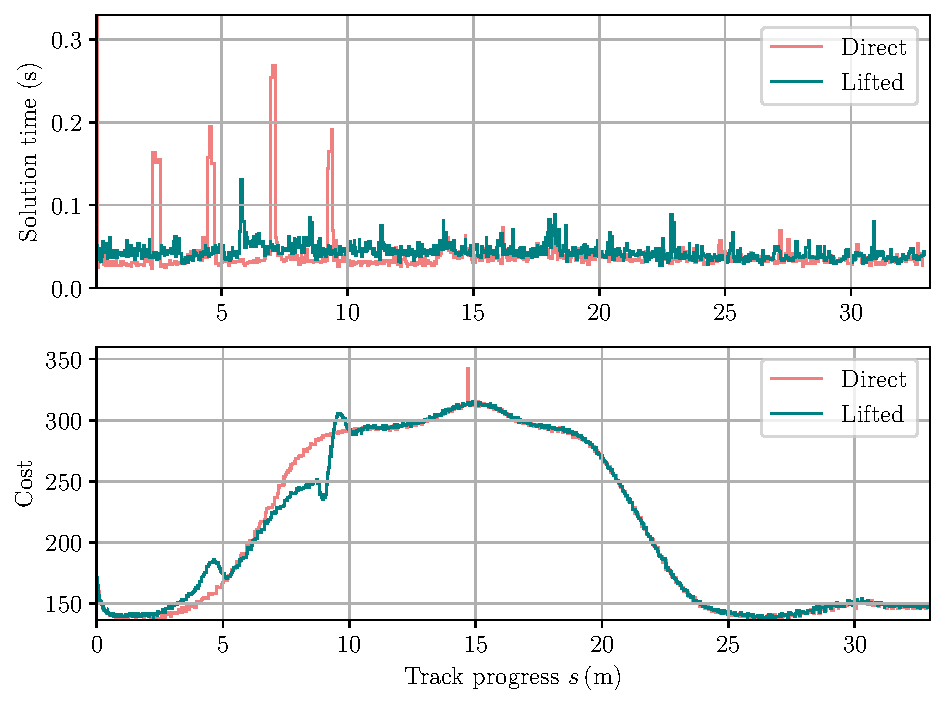
\includegraphics[scale=0.65]{figures/metrics}
		\end{figure}
	\end{column}
	\begin{column}{0.3\textwidth}
		\begin{table}[h!tbp]
			\small
			\begin{center}
				\begin{tabular}{lccccl}\toprule
					& $\tau_{\mathrm{rti,\,avg}}$\\
					\midrule
					$\mathrm{Direct}$& $39.90\,\mathrm{ms}$\\
					$\mathrm{Lifted}$& $43.92\,\mathrm{ms}$\\
					\bottomrule
				\end{tabular}
			\end{center}
			% \caption{Control oscillation metrics}
		\end{table}

		\begin{table}[h!tbp]
			\small
			\begin{center}
				\begin{tabular}{lccccl}\toprule
					& $\tau_{\mathrm{rti,\,max}}$\\
					\midrule
					$\mathrm{Direct}$& $269\,\mathrm{ms}$\\
					$\mathrm{Lifted}$& $134\,\mathrm{ms}$\\
					\bottomrule
				\end{tabular}
			\end{center}
			% \caption{Control oscillation metrics}
		\end{table}
	\end{column}
	\end{columns}
\end{frame}

\begin{frame}{Lifted $\zeta^{u}$, $u$ for AGV covering circles in the real warehouse}
	\begin{columns}[onlytextwidth]
		\begin{column}{0.75\textwidth}
	\begin{figure}[h!tbp]
		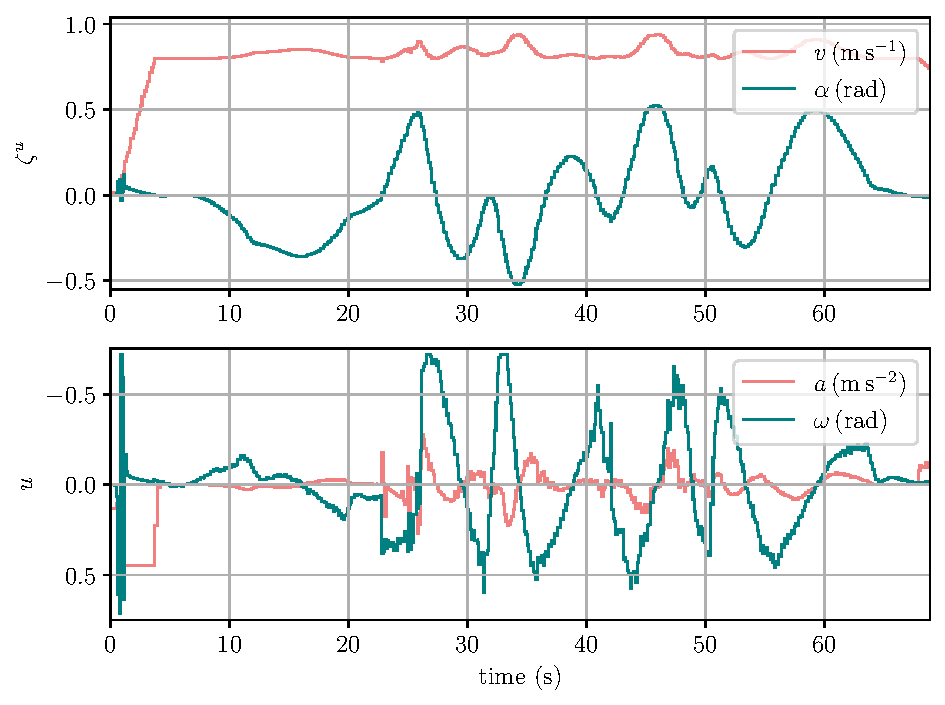
\includegraphics[scale=0.65]{figures/u_time}
		\end{figure}
	\end{column}
	\begin{column}{0.3\textwidth}
		\begin{table}[h!tbp]
			\small
			\begin{center}
				\begin{tabular}{lccccl}\toprule
					& $\tau_{\mathrm{rti,\,avg}}$\\
					\midrule
					$\mathrm{Direct}$& $28.99\,\mathrm{ms}$\\
					$\mathrm{Lifted}$& $30.99\,\mathrm{ms}$\\
					\bottomrule
				\end{tabular}
			\end{center}
			% \caption{Control oscillation metrics}
		\end{table}

		\begin{table}[h!tbp]
			\small
			\begin{center}
				\begin{tabular}{lccccl}\toprule
					& $\varepsilon_{\omega,\,\mathrm{osc}}\,(\mathrm{rad\,s^{-1}})$\\
					\midrule
					$\mathrm{Direct}$& $1.66\cdot10^{-1}$\\
					$\mathrm{Lifted}$& $2.86\cdot10^{-1}$\\
					\bottomrule
				\end{tabular}
			\end{center}
			% \caption{Control oscillation metrics}
		\end{table}
		\begin{table}[h!tbp]
			\small
			\begin{center}
				\begin{tabular}{lccccl}\toprule
					& $\varepsilon_{a,\,\mathrm{osc}}\,(\mathrm{m\,s^{-2}})$\\
					\midrule
					$\mathrm{Direct}$& $5.69\cdot10^{-2}$\\
					$\mathrm{Lifted}$& $9.52\cdot10^{-2}$\\
					\bottomrule
				\end{tabular}
			\end{center}
			% \caption{Control oscillation metrics}
		\end{table}

	\end{column}
\end{columns}
\end{frame}

% \begin{frame}{OCP comparison for AGV covering circles in the real warehouse}
% 	\begin{table}[h!tbp]
% 		\small
% 		\begin{center}
% 			\begin{tabular}{lccccl}\toprule
% 				\textbf{Metric} & \textbf{Direct} & \textbf{Lifted}\\
% 				\midrule
% 				$\varepsilon_{n, \mathrm{avg}}$& $3.828\cdot10^{-1}\mathrm{m}$& $4.688\cdot10^{-1}\mathrm{m}$\\
% 				$\tau_{\mathrm{rti,\,avg}}$& $2.899\cdot10^{-2}\mathrm{s}$& $3.099\cdot10^{-2}\mathrm{s}$\\
% 				\bottomrule
% 			\end{tabular}
% 		\end{center}
% 		\caption{Centreline deviation and solution timing}
% 	\end{table}
% 	\begin{table}[h!tbp]
% 		\small
% 		\begin{center}
% 			\begin{tabular}{lccccl}\toprule
% 				\textbf{Metric} & \textbf{Direct} & \textbf{Lifted}\\
% 				\midrule
% 				$\varepsilon_{v,\,\mathrm{osc}}$& $7.96\cdot10^{-2}\,\mathrm{m\,s^{-1}}$& $4.37\cdot10^{-2}\,\mathrm{m\,s^{-1}}$\\
% 				$\varepsilon_{a,\,\mathrm{osc}}$& $5.69\cdot10^{-2}\,\mathrm{m\,s^{-2}}$& $9.52\cdot10^{-2}\,\mathrm{m\,s^{-2}}$\\
% 				$\varepsilon_{\omega,\,\mathrm{osc}}$& $1.66\cdot10^{-1}\,\mathrm{rad\,s^{-1}}$& $2.86\cdot10^{-1}\,\mathrm{rad\,s^{-1}}$\\				
% 				\bottomrule
% 			\end{tabular}
% 		\end{center}
% 		\caption{Control oscillation metrics}
% 	\end{table}
% \end{frame}

\begin{frame}{Conclusion}
	\begin{itemize}[label=\textbullet]
	\item Successful deployment of 2 real time feasible trajectory tracking MPC schemes
	\item Covering circles perform better than severely nonlinear elliptical constraint
	\item Lifted has higher average solution time, but fewer maximum solution time overshoots
	\item Warehouse tests support real time optimality claim for lifted
	\end{itemize}
\end{frame}

\appendix
\begin{frame}
\end{frame}

\begin{frame}{Appendix: Measurement feedback loop}
	\begin{columns}[onlytextwidth]
		\begin{column}{0.5\textwidth}	
			\begin{table}[h!tbp]
				\small
				\begin{center}
					\begin{tabular}{lccccl}\toprule
						\textbf{Quantity} & \textbf{Value}\\
						\midrule
						sampling time $\tau_{s}$ &$60\,\mathrm{ms}$\\
						MPC deadline $\tau_{c}$ &$60\,\mathrm{ms}$ \\
						Measurement delay $\tau_{m}$ & $60\,\mathrm{ms}$  \\
						Actuation delay $\tau_{a}$ & $60\,\mathrm{ms}$ \\
						\bottomrule
					\end{tabular}
				\end{center}
				\caption{Timing parameters}
			\end{table}
		\end{column}

		\begin{column}{0.5\textwidth}
			\begin{center}
			\def\svgwidth{1.0\textwidth}
			\input{figures/state_observer.pdf_tex}
			\end{center}
		\end{column}
	\end{columns}
\end{frame}

\begin{frame}{Appendix: MPC parameters}
	\begin{columns}[onlytextwidth]
		\begin{column}{0.5\textwidth}	
		\begin{table}[h!tbp]
			\small
			\begin{center}
				\begin{tabular}{lccccl}\toprule
					\textbf{Quantity} & \textbf{Value}\\
					\midrule
					Shooting nodes $N$ & $150$ \\
					Reference progress $s_{\mathrm{ref}}$ & $1.2\cdot\,10^{1}\,\mathrm{m}$ \\
					Reference wheel speed $v_{\mathrm{ref}}$ & $8\cdot\,10^{-1}\,\mathrm{m\,s^{-1}}$\\
					\bottomrule
				\end{tabular}
			\end{center}
			\caption{Horizon parameters}
		\end{table}
		\end{column}
		\begin{column}{0.5\textwidth}	
			\begin{table}[h!tbp]
				\small
				\begin{center}
					\begin{tabular}{lccccl}\toprule
						\textbf{Lower bound} & \textbf{Value}\\
						\midrule
						$\underline{\dot{v}}$& -$5\cdot10^{-1}\,\mathrm{m\,s^{-2}}$ \\
						$\underline{\dot{\alpha}}$& -$8\cdot10^{-1}\,\mathrm{rad\,s^{-1}}$ \\
						$\underline{w}$ & -$1\,\mathrm{m\,s^{-1}}$ \\
						$\underline{\dot{\varphi}}$& -$5\cdot10^{-1}\,\mathrm{rad\,s^{-1}}$ \\
						\bottomrule
					\end{tabular}
				\end{center}
				\caption{Application layer thresholds}
			\end{table}
			\end{column}
	\end{columns}
\end{frame}		

\begin{frame}{Appendix: State $\zeta^{f}$ comparison for AGV covering circles in Gazebo}
	\begin{figure}[h!tbp]
		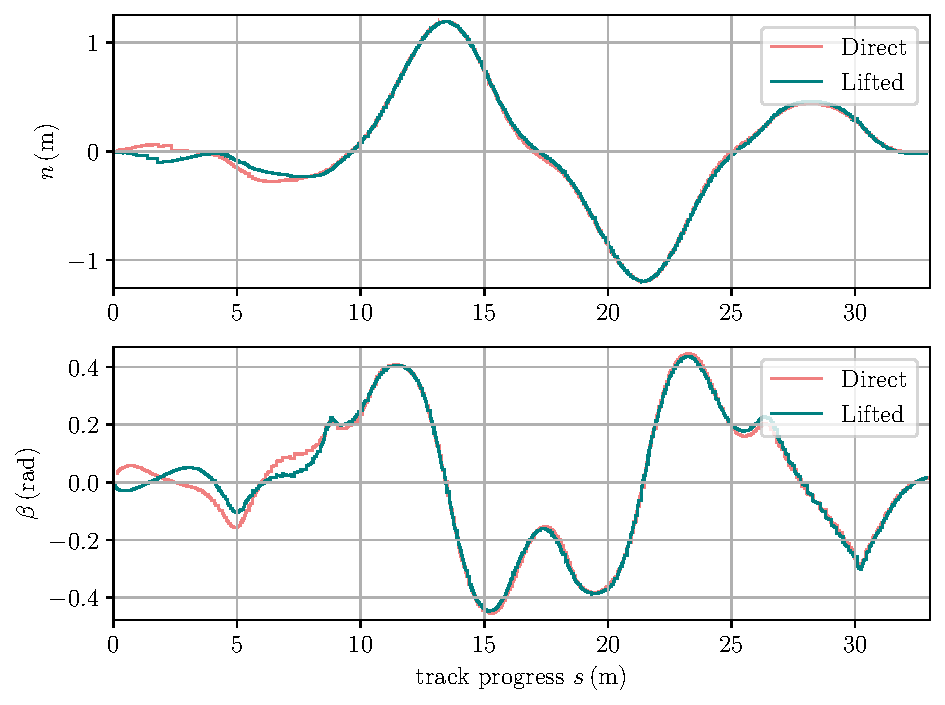
\includegraphics[scale=0.65]{figures/zeta_f}
	\end{figure}
\end{frame}

\begin{frame}{Appendix: State $\zeta^{u}$ comparison for AGV covering circles in Gazebo}
	\begin{figure}[h!tbp]
		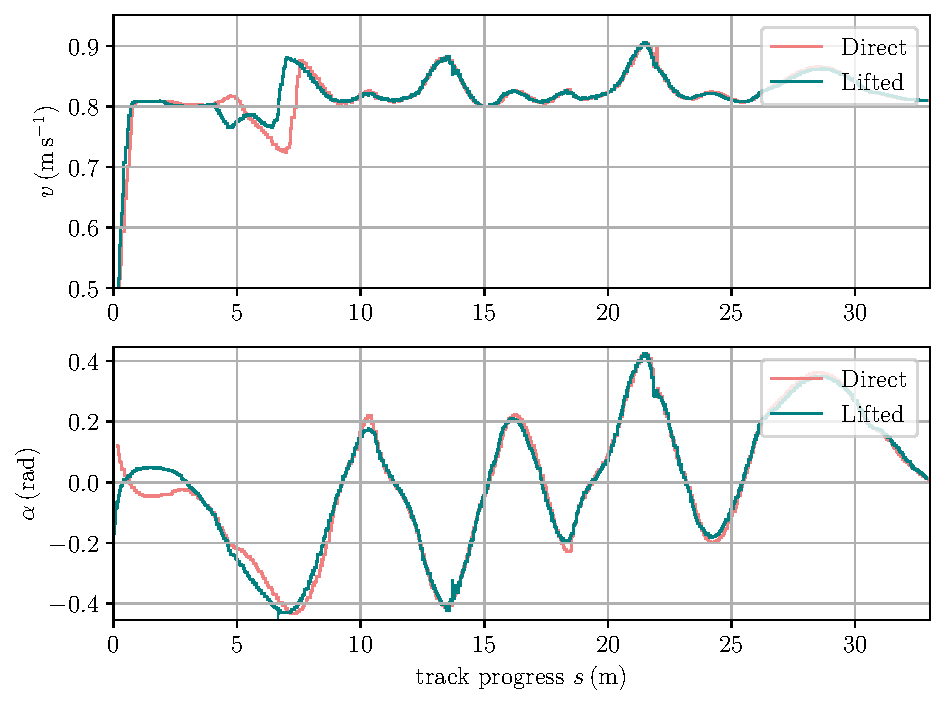
\includegraphics[scale=0.65]{figures/zeta_u}
	\end{figure}
\end{frame}

\begin{frame}{Appendix: Elliptical Footprint}
	\begin{columns}[onlytextwidth]
		\begin{column}{0.45\textwidth}
			\begin{center}
			\def\svgwidth{1.1\textwidth}
			\input{figures/agv_el2.pdf_tex}
			\end{center}
		\end{column}

		\begin{column}{0.45\textwidth}
			\begin{itemize}[label=\textbullet]
				\item ${i} \in [1, .., n_{ob}]$ circular obstacles
				\item ${k} \in [1, .., N]$ shooting nodes
			\end{itemize}
		\begin{align*}
			\begin{bmatrix}
				\Delta x_{i, k}\\
				\Delta y_{i, k}
			\end{bmatrix}^T
			\Sigma_{i}(\zeta_{k})
			\begin{bmatrix}
				\Delta x_{i, k}\\
				\Delta y_{i, k}
			\end{bmatrix} - 1 = 0
		\end{align*}

		\begin{align*}\Sigma_{i}(\zeta_{k}) =     
			\mathrm{M}(\varphi_{k})^T
			\begin{bmatrix}
				1/\lambda^{2}_{i} & 0\\
				0 & 1/\rho^{2}_{i}
			\end{bmatrix}
			\mathrm{M}(\varphi_{k})
		\end{align*}
		\end{column}
	\end{columns}
\end{frame}

\begin{frame}{Appendix: Control $u$ comparison for elliptical AGV footprint in Gazebo}
	\begin{columns}
	\begin{column}{0.75\textwidth}
	\begin{figure}[h!tbp]
		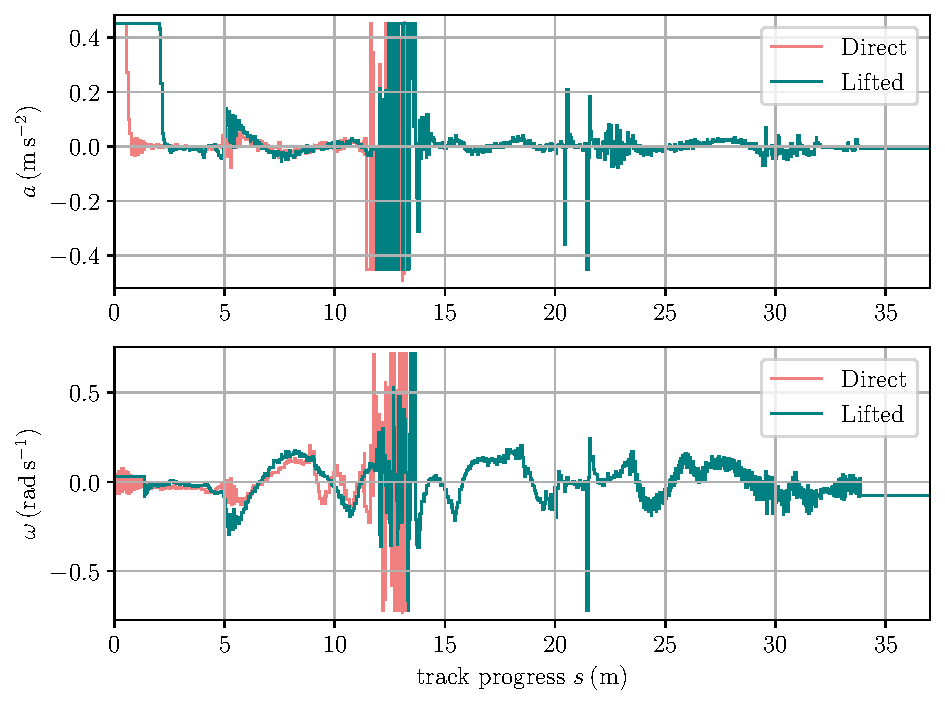
\includegraphics[scale=0.65]{figures/u_2c}
		% \caption{Comparison of the impact of the application software's control thresholding for different reference trajectory schemes.} \label{fig_ucomp_ref}
	\end{figure}
	\end{column}
	\begin{column}{0.3\textwidth}
		\begin{table}[h!tbp]
			\small
			\begin{center}
				\begin{tabular}{lccccl}\toprule
					& $\varepsilon_{a,\,\mathrm{osc}}\,(\mathrm{m\,s^{-2}})$\\
					\midrule
					$\mathrm{Direct}$& $7.95\cdot10^{-1}$\\
					$\mathrm{Lifted}$& $2.67\cdot10^{-1}$\\
					\bottomrule
				\end{tabular}
			\end{center}
			% \caption{Control oscillation metrics}
		\end{table}

		\begin{table}[h!tbp]
			\small
			\begin{center}
				\begin{tabular}{lccccl}\toprule
					& $\varepsilon_{\omega,\,\mathrm{osc}}\,(\mathrm{rad\,s^{-1}})$\\
					\midrule
					$\mathrm{Direct}$& $9.90\cdot10^{-2}$\\
					$\mathrm{Lifted}$& $1.78\cdot10^{-2}$\\
					\bottomrule
				\end{tabular}
			\end{center}
			% \caption{Control oscillation metrics}
		\end{table}
	\end{column}
\end{columns}
\end{frame}

\begin{frame}{Appendix: State$\varphi,\,n$ comparison for elliptical AGV footprint in Gazebo}
	\begin{columns}
		\begin{column}{0.7\textwidth}
	\begin{figure}[h!tbp]
	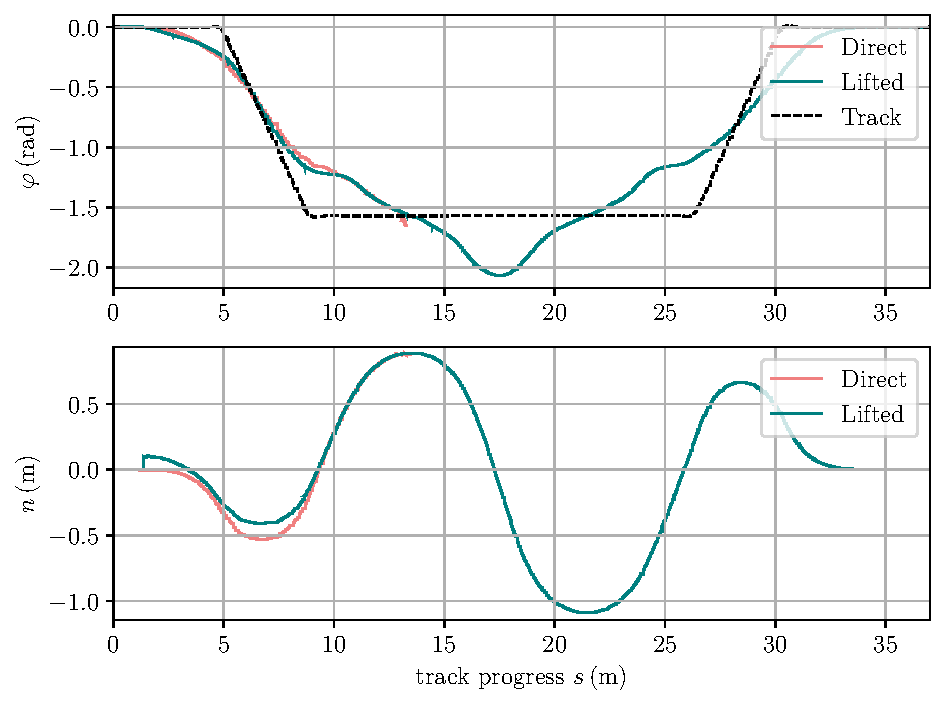
\includegraphics[scale=0.65]{figures/zeta_phi_n_el}
	% \caption{Comparison of the impact of the application software's control thresholding for different reference trajectory schemes.} \label{fig_ucomp_ref}
\end{figure}
\end{column}
\begin{column}{0.3\textwidth}
	\begin{table}[h!tbp]
		\small
		\begin{center}
			\begin{tabular}{lccccl}\toprule
				& $\varepsilon_{n,\,\mathrm{avg}}\,(\mathrm{m})$\\
				\midrule
				$\mathrm{Direct}$& $6.78\cdot10^{-1}$\\
				$\mathrm{Lifted}$& $4.67\cdot10^{-1}$\\
				\bottomrule
			\end{tabular}
		\end{center}
		% \caption{Control oscillation metrics}
	\end{table}
\end{column}
\end{columns}
\end{frame}

\begin{frame}{Appendix: State $x,\,y$  comparison for elliptical AGV footprint in Gazebo}
	\begin{figure}[h!tbp]
		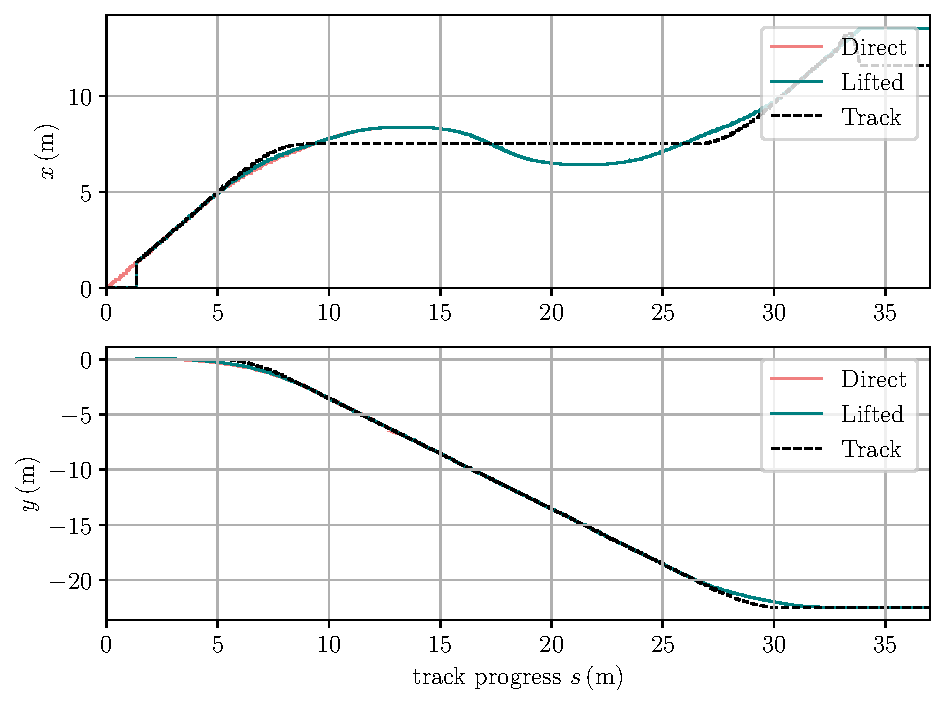
\includegraphics[scale=0.65]{figures/zeta_c_el}
		% \caption{Comparison of the impact of the application software's control thresholding for different reference trajectory schemes.} \label{fig_ucomp_ref}
	\end{figure}
\end{frame}

\begin{frame}{Appendix: State $\zeta^{u}$ comparison for elliptical AGV footprint in Gazebo}
	\begin{figure}[h!tbp]
		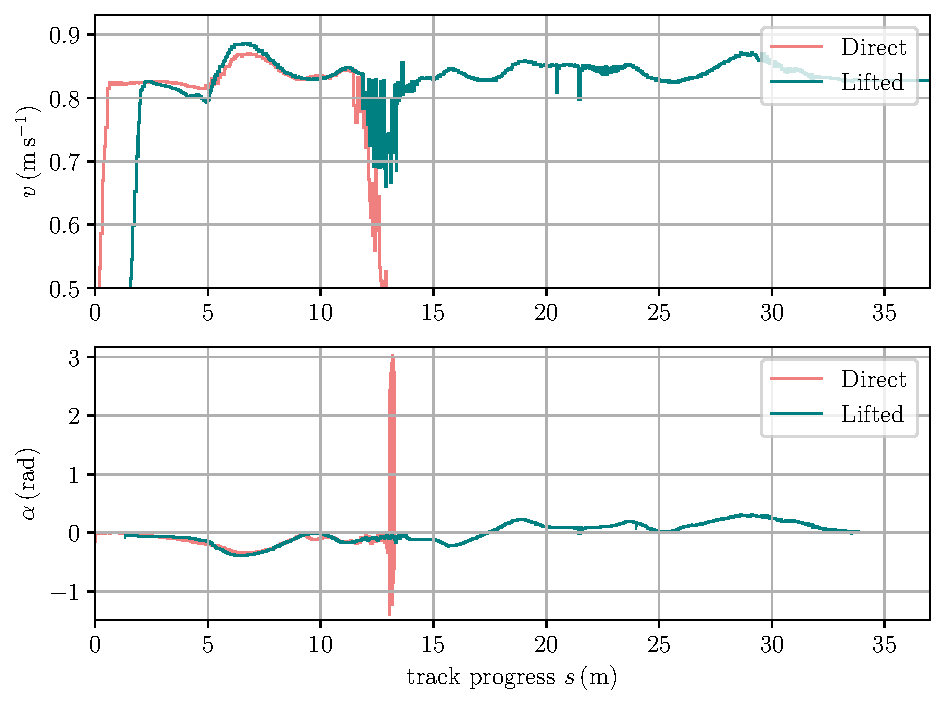
\includegraphics[scale=0.65]{figures/zeta_u_2c}
		% \caption{Comparison of the impact of the application software's control thresholding for different reference trajectory schemes.} \label{fig_ucomp_ref}
	\end{figure}
\end{frame}

% \begin{frame}{Appendix: State $\zeta^{f}$ comparison for elliptical AGV footprint in Gazebo}
% 	\begin{figure}[h!tbp]
% 		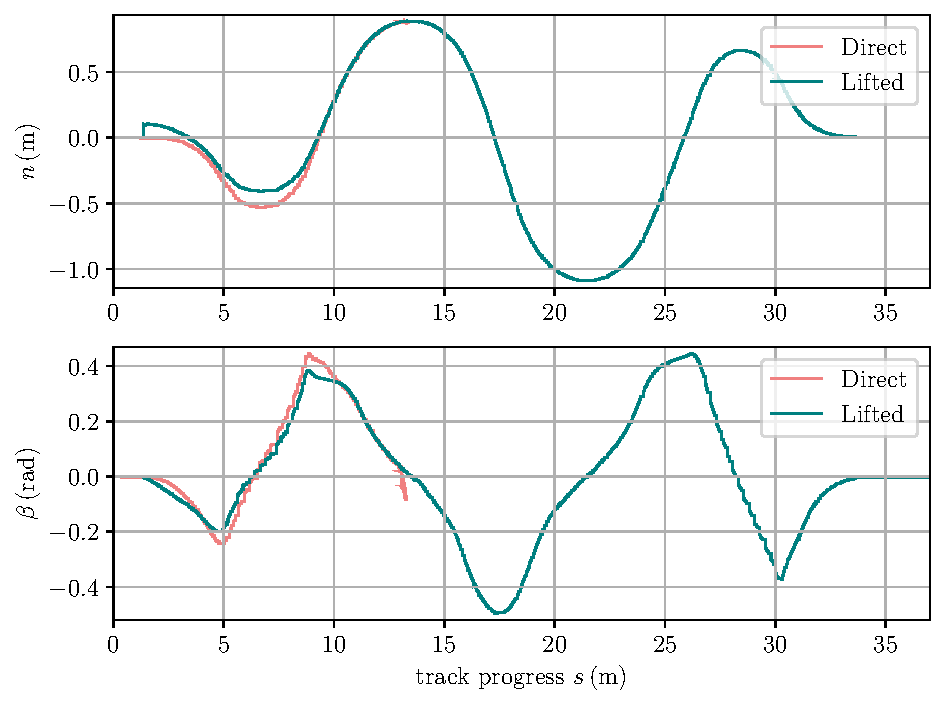
\includegraphics[scale=0.65]{figures/zeta_f_2c}
% 		% \caption{Comparison of the impact of the application software's control thresholding for different reference trajectory schemes.} \label{fig_ucomp_ref}
% 	\end{figure}
% \end{frame}

\begin{frame}{Appendix: Delay compensation comparison in Gazebo}
	\begin{figure}[h!tbp]
		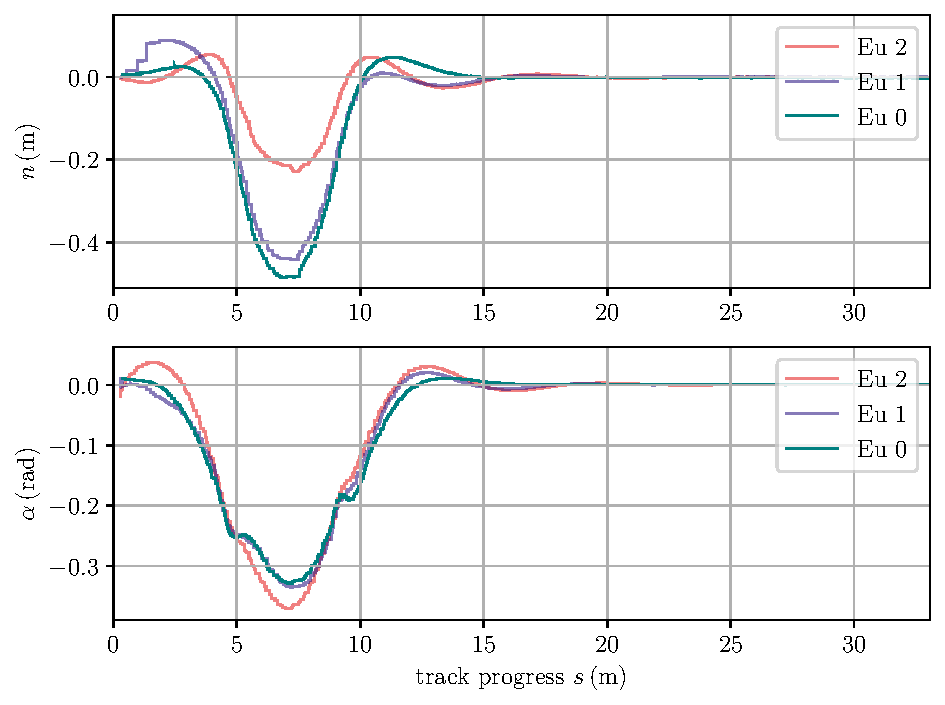
\includegraphics[scale=0.65]{figures/predictor}
		% \caption{Comparison of the impact of the application software's control thresholding for different reference trajectory schemes.} \label{fig_ucomp_ref}
	\end{figure}
\end{frame}

\begin{frame}{Appendix: Lifted $\zeta^{c}$, $\zeta^{u}$ for AGV covering circles in the real warehouse}
	\begin{figure}[h!tbp]
		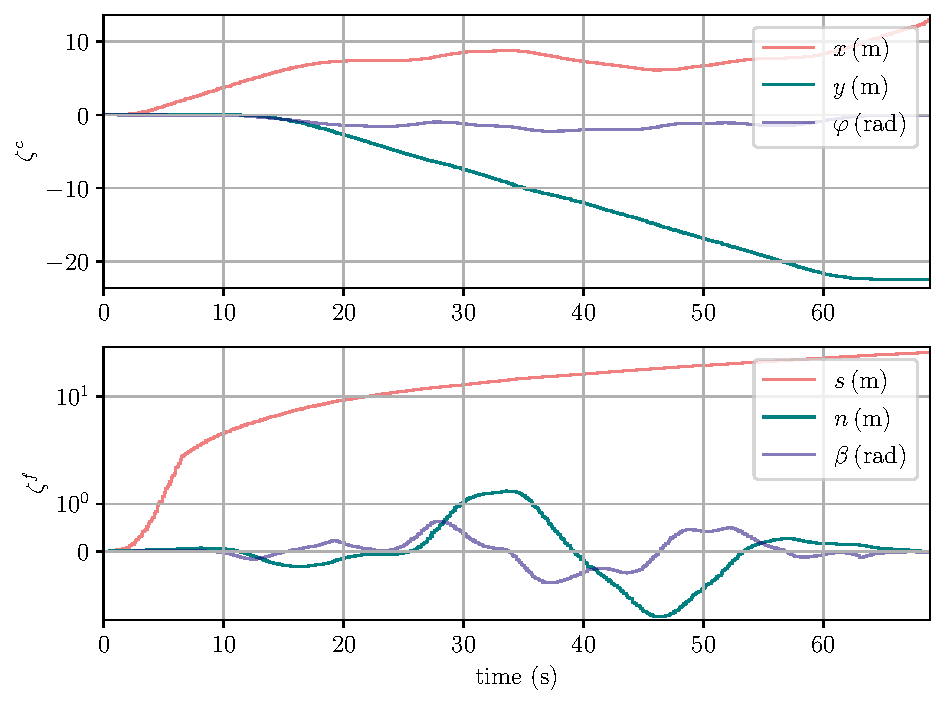
\includegraphics[scale=0.65]{figures/zeta_time}
	\end{figure}
\end{frame}

\begin{frame}{Appendix: Control software architecture}
	\begin{columns}[onlytextwidth]
	\begin{column}{0.95\textwidth}
	\begin{center}
		\def\svgwidth{0.85\textwidth}
		\input{figures/control_archi.pdf_tex}
		\end{center}

	\end{column}

	\begin{column}{0.05\textwidth}
		\begin{align*}
			\eta =\begin{bmatrix}
				w\\
				\dot{\varphi}
			\end{bmatrix} 
			% &= 
			% \begin{bmatrix}
			% 	v\, \cos(\alpha)\\
			% 	\dfrac{v}{d}\, \sin(\alpha)\label{twist}
			% \end{bmatrix}
		\end{align*}
	\end{column}
\end{columns}
\end{frame}

\begin{frame}{Future Scope}
	\begin{itemize}[label=\textbullet]
	\item Extend geometric constraint to more shapes.
	\item Improve obstacle estimation.  
	\item Investigate other stablization schemes for reduced DAE system.
	\end{itemize}
\end{frame}

\end{document}